\documentclass[12pt]{article}

\usepackage{geometry}
\geometry{a4paper, left=1in, right=1in, top=1in, bottom=1in}
\usepackage{amsmath}
\usepackage{amsmath,amsfonts,amssymb}
\usepackage{graphicx}
\usepackage{enumitem}
\usepackage{titlesec}
\usepackage{fancyhdr}
\usepackage{hyperref}
\usepackage{floatrow}

\begin{document}
\textbf{(a)} The images were read using the imread function (and cast as double). Then we took 12 pairs of point as input from the user (through mouse click). The points were choosen to be as accurate and similar as possible. The values were saved in ``selected\_points.mat" to save effort for further runs. Here is a small section of the code:
\begin{verbatim}
n = 12; % Number of points
for i=1:n
    figure(1); 
    imshow(im1/255); 
    [x1(i), y1(i)] = ginput(1);
    figure(2); 
    imshow(im2/255); 
    [x2(i), y2(i)] = ginput(1);
end
save(`selected_points.mat', `x1', `y1', `x2', `y2');
\end{verbatim}


\textbf{(b)}
We consider that the affine transformation matrix will be of the form:
\[
    \begin{bmatrix}
        x_1 & x_2 & x_3 \\
        x_4 & x_5 & x_6 \\
        0 & 0 & 1
    \end{bmatrix}
\]

We initialize matrix A with points from Img1 (n = 12 in our case):
\[
    \begin{bmatrix}
        x_{11} & x_{12} & x_{13} & \dots & x_{1n} \\
        y_{11} & x_{12} & y_{13} & \dots & y_{1n} \\
        1 & 1 & 1 & \dots & 1
    \end{bmatrix}
\]

Similarly, we initialize matrix b with points from Img2:
\[
    \begin{bmatrix}
        x_{21} & x_{22} & x_{23} & \dots & x_{2n} \\
        y_{21} & x_{22} & y_{23} & \dots & y_{2n} \\
        1 & 1 & 1 & \dots & 1
    \end{bmatrix}
\]
The equation which we need to solve finally is (using least squares approach, since these are not square matrices):
\[TA = b\]


\textbf{(c)}
In this part, we used nearest neighbour interpolation for image warping. We used reverse warping (which gives better results than forward warping). We initialized a matrix of size same as Img2 with zeroes. We then iterated over the points and calculated the their corresponding point using the inverse of matrix T (already obtained from previous part). Then, the values obtained were rounded, and also, we considered only those values which were in bounds. Here is the code:
\begin{verbatim}
warpedImg = zeros(size(im2), 'uint8');
for r = 1:size(im2, 1)
    for c = 1:size(im2, 2)
        originalCoords = invT * [c; r; 1];
        xOriginal = originalCoords(1);
        yOriginal = originalCoords(2);
        xNearest = round(xOriginal);
        yNearest = round(yOriginal);
        if xNearest >= 1 && xNearest <= cols && yNearest >= 1 && yNearest <= rows
            warpedImg(r, c, :) = im1(yNearest, xNearest, :);
        end
    end
end
\end{verbatim}

Here are all the three images displaeyed:

\begin{figure}[h]
    \centering
    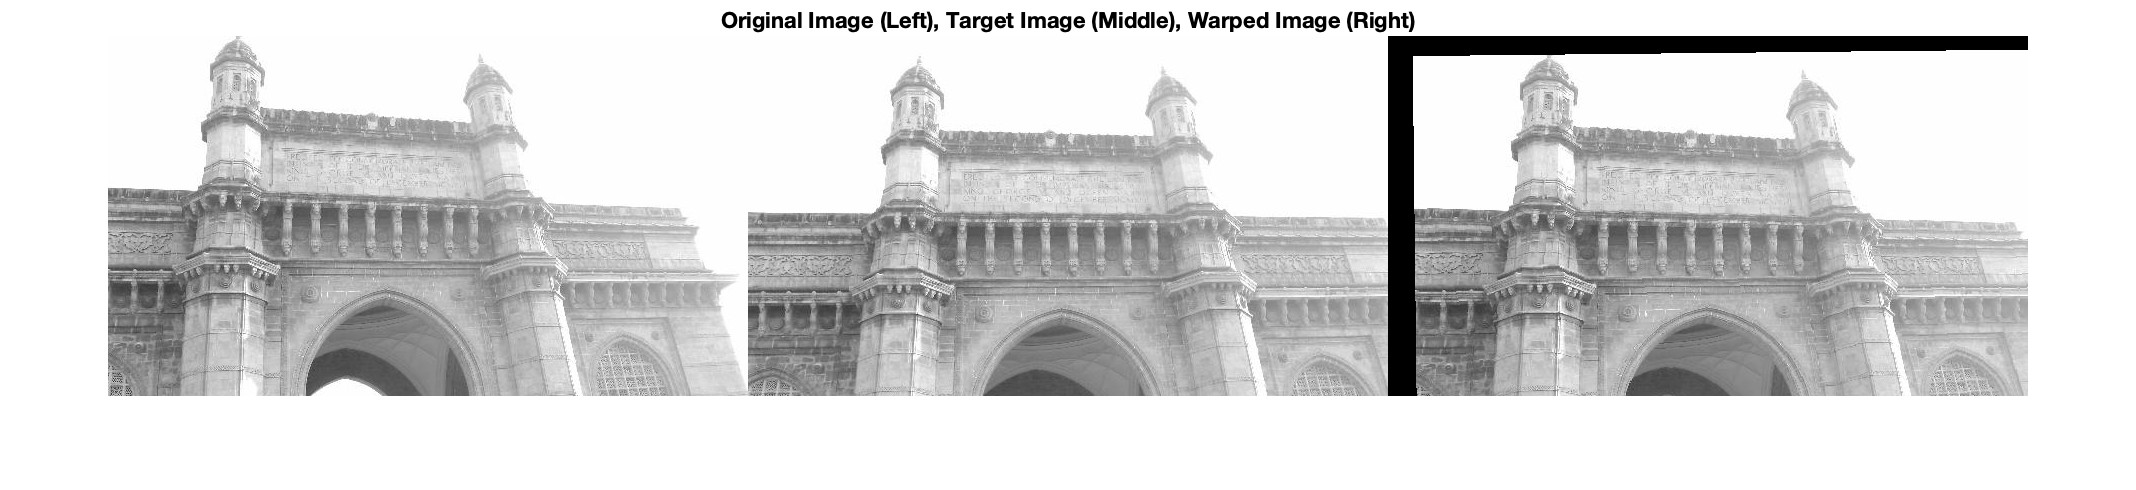
\includegraphics[width=\linewidth]{nearest.jpg}
    \caption{Image warped using nearest neighbour interpolation}
\end{figure}

As we can see, the third image looks quite similar and aligned to the second image (except the black border, which comes because of out of bound values when multiplying by inv(T)).


\textbf{(d)}
In this part, we used bilinear interpolation for image warping. The approach looks similar to the previous part, but instead of mapping the intensities to nearest integral points, we consider the weighted average of all 4 neighbouring points. And the weights are the areas of the four rectangles, here is the code:
\begin{verbatim}
    for r = 1:size(im2, 1)
    for c = 1:size(im2, 2)
        originalCoords = invT * [c; r; 1];
        xOriginal = originalCoords(1);
        yOriginal = originalCoords(2);
        x1 = floor(xOriginal);
        y1 = floor(yOriginal);
        x2 = x1 + 1;
        y2 = y1 + 1;
        dx = xOriginal - x1;
        dy = yOriginal - y1;
        pixelValue = zeros(1, channels);
        if x1 >= 1 && x1 <= cols && y1 >= 1 && y1 <= rows
            pixelValue = (1-dx)*(1-dy)*double(im1(y1, x1, :));
        end
        if x2 >= 1 && x2 <= cols && y1 >= 1 && y1 <= rows
            pixelValue = pixelValue + dx*(1-dy)*double(im1(y1, x2, :));
        end
        if x1 >= 1 && x1 <= cols && y2 >= 1 && y2 <= rows
            pixelValue = pixelValue + (1-dx)*dy*double(im1(y2, x1, :));
        end
        if x2 >= 1 && x2 <= cols && y2 >= 1 && y2 <= rows
            pixelValue = pixelValue + dx*dy*double(im1(y2, x2, :));
        end
        warpedImg(r, c, :) = uint8(pixelValue);
    end
end   
\end{verbatim} 
\begin{figure}[h]
    \centering
    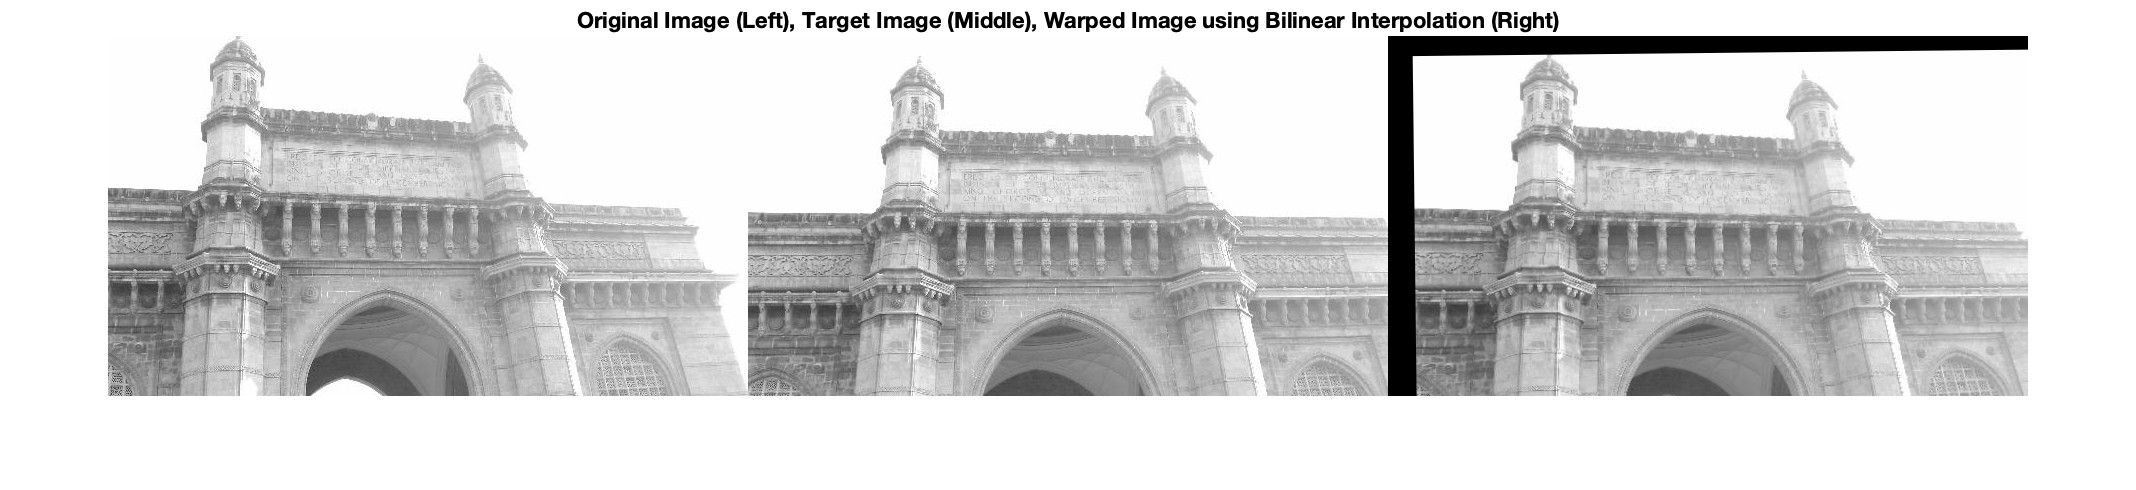
\includegraphics[width=\linewidth]{bilinear.jpg}
    \caption{Image warped using bilinear interpolation}
\end{figure}
Similar to the previous case, the image aligns really well.

\textbf{(e)}
We already know that A is of the form:
\[
    \begin{bmatrix}
        x_{11} & x_{12} & x_{13} & \dots & x_{1n} \\
        y_{11} & x_{12} & y_{13} & \dots & y_{1n} \\
        1 & 1 & 1 & \dots & 1
    \end{bmatrix}
\]
and b is of the form:
\[
    \begin{bmatrix}
        x_{21} & x_{22} & x_{23} & \dots & x_{2n} \\
        y_{21} & x_{22} & y_{23} & \dots & y_{2n} \\
        1 & 1 & 1 & \dots & 1
    \end{bmatrix}
\]

It has also been given that the control points are perfectly colinear i.e. $y_{1i} = mx_{1i}+c$. 
\[b = TA\]
\[bA^T = TAA^T\]
where $A^T$ is the transpose of matrix A. We can fine $T$ if $AA^T$ is invertible. $P = AA^T$ is given by:
\[
    \begin{bmatrix}
        \sum_{i=1}^nx_{1i}^2 & a\sum_{i=1}^nx_{1i}^2 + b\sum_{i=1}^nx_{1i} & \sum_{i=1}^nx_{1i}\\
        a\sum_{i=1}^nx_{1i}^2 + b\sum_{i=1}^nx_{1i} &  a^2\sum_{i=1}^nx_{1i}^2 + 2ab\sum_{i=1}^nx_{1i} + kb^2 & a\sum_{i=1}^nx_{1i} + nb\\
        \sum_{i=1}^nx_{1i} & a\sum_{i=1}^nx_{1i} + nb & n
    \end{bmatrix}
\]

If $C_1, C_2, C_3$ are the columns of the matrix $P$, then we can see from above that $C_2 - aC_1 - bC_3 = 0$. Hence the matrix is not invertible (rank-deficient). Hence, we will not be able to find $T$ using this method. Hence, affine transformation cannot be used if we choose co-linear points.
\end{document}